\clearpage

\section{Continuity}

\subsection{The big picture}

Let \((\mc{X},\ms{T}_{\mc{X}})\), \((\mc{Y},\ms{T}_{\mc{Y}})\), \((\mc{Z},\ms{T}_{\mc{Z}})\) be HTS's.
\begin{ndef}{: Continuous}
	Let \(f:\mc{X}\to\mc{Y}\) be a (single valued) mapping. To call \(f\) \emph{\textbf{continuous}} (on \((\mc{X},\ms{T}_{\mc{X}})\)) means for all \(\mc{G}\in\ms{T}_{\mc{Y}}\), \(f^{-1}(\mc{G})\in\ms{T}_{\mc{X}}\), i.e., every open set \(\mc{G}\) in \(\mc{Y}\) has an open pre-image \(f^{-1}(\mc{G})=\{x\in\mc{X}\st f(x)\in\mc{G}\}\).
\end{ndef}
\begin{example}
	For any metric space \((\mc{X},d)\) with \(p\in\mc{X}\), the function \(f:\mc{X}\to\R\) such that \(f(x)=d(x,p)\) is continuous.
\end{example}
\begin{proof}[Proof sketch]
	Given open \(\mc{G}\subseteq\R\), consider \(f^{-1}(\mc{G})\), a set in \(\mc{X}\). E.g., if \(\mc{G}=(a,b)\), and \(a\geq 0\), 
	\begin{align*}
		f^{-1}((a,b))=&\{x\in\mc{X}:a<d(x,p)<b\}\\
		=&\B[p;b)\backslash\B[p;a]\\
		=&\B[p;b)\cap(\B[p;a])^c,
	\end{align*}
	which is an intersection of two open sets, hence open. Rest of the proof is left as an exercise.
	\begin{figure}[htb]
		\centering
		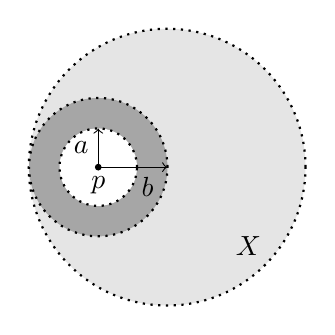
\begin{tikzpicture}
			\draw[dotted, thick, fill = white!60!lightgray] (0,0) circle (50pt);
			\draw[dotted, thick, fill = lightgray!60!gray] (-0.875,0) circle (25pt);
			\draw[dotted, thick, fill = white!60!white] (-0.875,0) circle (14pt);
			\draw[fill] (-0.875,0) circle (1pt);
			\node[below] at (-0.875,0) {\(p\)};
			\draw[->] (-0.875,0)--(0,0);
			\draw[->] (-0.875,0)--(-0.875,0.49);
			\node[left] at (-0.875, 0.245) {\(a\)};
			\node[below] at (-0.25,0) {\(b\)};
			\node[right] at (0.75, -1) {\(\mc{X}\)};
		\end{tikzpicture}
		\caption{Visualization of the pre-image in the proof above.}
	\end{figure}
\end{proof}
\begin{note}
	Continuity does not allow functions with ``holes" to exist: something that you have probably seen before in MATH 100 or equivalent courses.
\end{note}
\begin{nproposition}{: Continuity and Density}
	Given \(f_1,f_2:\mc{X}\to\mc{Y}\) both continuous, and some set \(\mc{Q}\subseteq\mc{X}\),
	\begin{equation*}
		f_1(q)=f_2(q)~\text{for all}~q\in\mc{Q}\implies f_1(q)=f_2(q)~\text{for all}~q\in\ol{\mc{Q}}.
	\end{equation*}
\end{nproposition}
\begin{proof}
	Pick any \(x\in\ol{\mc{Q}}\) and let \(y_1=f_1(x)\), \(y_2=f_2(x)\). We shall show that \(y_1=y_2\). Pick any open neighbourhoods \(\mc{U}_1\in\ms{N}(y_1)\), \(\mc{U}_2\in\ms{N}(y_2)\) such that 
	\begin{equation*}
		\Omega_1=f^{-1}_1(\mc{U}_1),~\Omega_2=f^{-1}_2(\mc{U}_2)
	\end{equation*}
	are open by continuity. Let \(\Omega=\Omega_1\cap\Omega_2\); clearly \(x\in\Omega\), so since \(x\in\ol{\mc{Q}}\), \(\Omega\cap\mc{Q}\neq\emptyset\).
	\begin{figure}[htbp]
		\centering
		\begin{tikzpicture}
			\draw[dotted, very thick, color=red] (0.924,1.71) to [curve through = {(0.308,1.519) ..(0,1.414)..(-2,0)..(0,-1.414)..(0.308,-1.519)}] (0.924,-1.71);
			\draw[dotted, very thick, color=blue] (0,1.826) to [curve through = {(0.308,1.519)..(1,0)..(0.308,-1.519)}] (0,-1.826);
			\draw[fill] (0,0) circle (1pt);
			\node[below] at (0,0) {\(x\)};
			\node[below] at (0.924,1.71) {\(\color{red} \Omega_2\)};
			\node[left] at (0,-1.826) {\(\color{blue} \Omega_1\)}; 
		\end{tikzpicture}
		\caption{Visualization of the proof.}
	\end{figure}
	Thus, for any \(q\in\Omega\cap\mc{Q}\), \(f_1(q)=f_2(q)\), and this point lies in \(\mc{U}_1\cap\mc{U}_2\). However, this shows that for all \(\mc{U}_1\in\ms{N}(y_1)\), \(\mc{U}_2\in\ms{N}(y_2)\), \(\mc{U}_1\cap\mc{U}_2\neq\emptyset\). Finally, all that remains is to compare HTS: the negation of this reveals that \(y_1=y_2\)
\end{proof}
\subsection{Continuity and Compactness}
\begin{ntheorem}{}
	Suppose \(\mc{X}\) is a \emph{compact} HTS, and \(f:\mc{X}\to\mc{Y}\) is continuous (on \(\mc{X}\)), then \(f(\mc{X})=\{f(x)\st x\in\mc{X}\}\) is compact in \(\mc{Y}\).
\end{ntheorem}
\begin{proof}
	Let \(\ms{G}\) be an arbitrary open cover for \(f(\mc{X})\). We construct \(\ms{G}_0=\{f^{-1}(\mc{G})\st \mc{G}\in\ms{G}\}\). Each element in \(\ms{G}_0\) is \emph{open} by continuity of \(f\), and clearly each \(x\in\mc{X}\) is in at least one \(\mc{G}\), so \(\mc{G}_0\) is an open cover of \(\mc{X}\). Compactness of \(\mc{X}\) guarantees that for some \(N\in\N\), \(f^{-1}(\mc{G}_1),f^{-1}(\mc{G}_2),\dots, f^{-1}(\mc{G}_N)\) form a finite subcover for \(\mc{X}\). In turn, this would mean that \(\mc{G}_1,\mc{G}_2,\dots,\mc{G}_N\) is an open subcover of \(f(\mc{X})\) selected from \(\ms{G}\). 
\end{proof}
\begin{note}[Consequences]
	For continuous \(f:\mc{X}\to\mc{Y}\) and \(\mc{X}\neq\emptyset\) compact, 
	\begin{enumerate}[(1)]
		\item If \(\mc{Y}\) is a metric space, \(f(\mc{X})\) is closed and compact.
		
		\item If \(\mc{Y}=\R\), then \(f(\mc{X})\) \emph{includes} the numbers \(\inf{f(\mc{X})}\), \(\sup{f(\mc{X})}\), i.e., \(\mc{X}\) contains points \(\ul{x},\ol{x}\in\mc{X}\) obeying \(f(\ul{x})\leq f(x)\leq f(\ol{x})\), for all \(x\in\mc{X}\), where \(\ul{x}:=\text{min}\{f(x)\}_{x\in\mc{X}}\) and \(\ol{x}:=\text{max}\{f(x)\}_{x\in\mc{X}}\).
	\end{enumerate}
\end{note}

\begin{ntheorem}{: Inverse mappings}
	Suppose \(\mc{X}\) is compact and \(f:\mc{X}\to\mc{Y}\) is bijective and continuous. Then, \(f^{-1}:\mc{Y}\to\mc{X}\) is continuous.
\end{ntheorem}
\begin{proof}
	For simplicity, let \(h=f^{-1}\). To check continuity, we show one of two equivalent statements:
	\begin{enumerate}[(i)]
		\item \(h^{-1}(\mc{U})\) is \emph{open} for any \emph{open} \(\mc{U}\subseteq\mc{X}\).
		
		\item \(h^{-1}(\mc{C})\) is \emph{closed} for any \emph{closed} \(\mc{C}\subseteq\mc{X}\).
	\end{enumerate}
	For this proof, we will show (ii): if \(\mc{C}\subseteq\mc{X}\) is closed, 
	\begin{align*}
		h^{-1}(\mc{C})=&\{y\in\mc{Y}\st h(y)\in\mc{C}\}\\
		=&\{y\in\mc{Y}\st f^{-1}(y)\in\mc{C}\}\\
		=&\{y\in\mc{Y}\st y\in f(\mc{C})\}=f(\mc{C});
	\end{align*}
	however, from our hypothesis, \(\mc{C}\) is compact, so \(f(\mc{C})\) is compact, hence closed.
\end{proof}